\documentclass[letterpaper,12pt]{article}

\RequirePackage{comment}
\RequirePackage[hypertex]{hyperref}
\RequirePackage{GE05}
% this inputs graphicx, too

\newcommand{\NX}{\mbox{\em NX\/}}
\newcommand{\POP}{\mbox{\em POP\/}}

\def\ClassName{The Global Economy}
\def\Category{Professor David Backus}
\def\HeadName{Midterm Exam}

\begin{document}
\parindent = 0.0in
\parskip = \bigskipamount
\thispagestyle{empty}%
\Head

\centerline{\large \bf \HeadName}%
%\centerline{March 9, 2005}
\centerline{Revised:  \today}

\bigskip
You have 75 minutes to complete this exam.  Please answer each
question in the space provided. You may consult one page of notes
and a calculator, but devices capable of wireless transmission are
prohibited.

I understand that the honor code applies: I will not lie, cheat,
or steal to gain an academic advantage, or tolerate those who do.

\begin{flushright}
\rule{4in}{0.5pt} \\ (Name and Signature)
\end{flushright}

\begin{figure}[h]
    \centering
    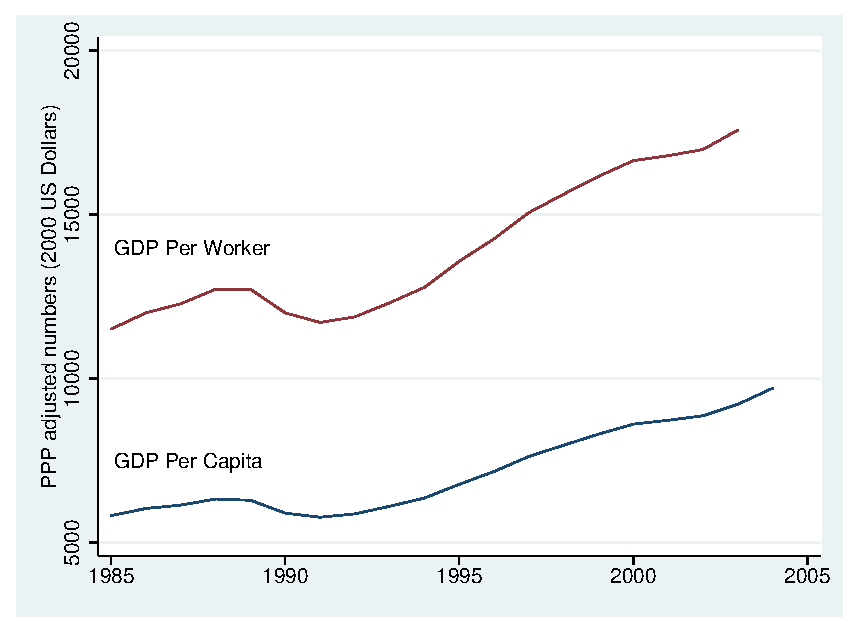
\includegraphics[scale=0.8]{pwtpolypopyl.eps}
    \caption{GDP Per Capita and GDP Per Worker in Poland.}
    \label{fig:mexico}
\end{figure}

\begin{enumerate}
% ======================================================================
\item {\it Poland emerges.\/} 
Poland's chaotic history stems largely from its unfortunate
location between Germany and Russia.  

Like many developing countries, 
Mexico followed a policy of ``import substitution'' after World War II, 
using high tariffs to help local industry ``substitute'' 
local products for imports.  
Trade policy changed dramatically in 1994,
when Mexico signed the North American Free Trade Agreement (NAFTA)
with Canada and the United States.
Under NAFTA, tariffs between these countries fell on a wide range 
of products and the volume of trade expanded rapidly.  
The question is how the change in policy affected overall 
economic performance.  
 
 %
 \begin{table}
    \centering 
    \tabcolsep = 0.2in
    \begin{tabular}{lccc}
    \hline\hline
    Year    &  $Y/\POP $  &  $Y/L$  &  $K/L$  \\
    \hline\hline
    1950 &  2,709 &  8,358   &  10,066 \\
    1980 &  7,271 &  23,360  &  48,334  \\
    1994 &  7,328 &  18,943  &  45,444 \\
    2003 &  7,938 &  18,628  &  47,089 \\
    \hline\hline
    \end{tabular}
    \caption{Output and Capital in Mexico.
    Data from the Penn World Tables.  Output (GDP) and capital
    are measured in 2000 US dollars.}
    \label{tab:mexico}    
\end{table}

%
Looking at Figure \ref{tab:mexico}, you decide to look at two periods, 
1950-80 and 1994-2003, throwing out the lost decade of the 1980s 
(a story for another time).  
In the first period, tariffs were high, in the second, much lower.  
Using the data provided and your own analytical skills, you decide to 
examine the impact of trade policy and the performance 
of Mexico's economy.  

\begin{enumerate}

\item How do growth in GDP per capita ($Y/\POP$) 
and GDP per worker ($Y/L$) differ between the two periods?  
What is the source of any differences between the two measures?    
(10~points)

\item What are the sources of growth in GDP per worker 
in the two periods?  
Note specifically growth in (total factor) productivity.  
(20~points)

\item How would you expect a reduction in trade barriers  
to affect productivity?
Is that what you see?  
Speculate on why or why not.   
(10~points)
\end{enumerate}


%\begin{comment}
Answer.
\begin{enumerate}

\item We compute continuously-compounded growth rates the usual way.
For GDP per capita, the growth rates 
are 3.29 (1950-80) and 0.89 (1994-2003).  
Both are expressed as percentages.
For GDP per worker, the growth rates are 3.43 and $-0.89$, respectively.  
With both measures, growth is much slower in the later period.  
The difference has to come from differences in the growth rates 
of population and workers; equivalently, the ratio of 
of workers to population must be changing.  

Grading:  8 points for computing the growth rates, 
2 for understanding the difference between them.  

\item The usual growth accounting exercise.  
Our decomposition of the growth rate of output per worker is 
\[
        \gamma_{Y/L} \;=\; \gamma_A + \alpha \gamma_{K/L}  
\]
with $\alpha = 1/3$.
The letter $A$ stands for total factor productivity (TFP).    
For the two periods, we get 
\begin{eqnarray*}
    \mbox{1950-1980:} &&  3.43  \;=\; 1.68 \mbox{ (A)} 
                +  1.74 = 5.23/3 \mbox{ (K/L)}   \\
    \mbox{1994-2003:} &&  -0.19 \;=\; -0.32 \mbox{ (A)} 
                +  0.13 \mbox{ (K/L)} .
\end{eqnarray*}
There's apparently a drop in TFP growth ($\gamma_A$).  

Grading: 20 points for getting the numbers exactly right, 
partial credit for other answers.  

\item This is the issue:  we have seen that reducing trade barriers
is like increasing TFP.  
But here we see that TFP fell during the period when trade 
barriers were lowest and trade was highest.  
What went wrong?  
One possibility is that the theory of trade is wrong:  
trade doesn't increase productivity.
Another is that something else is going on:  
the crisis in 1994-95 evident in the figure, 
some problem that inhibits the reallocation 
called for by trade (frictions 
in labor or capital markets?), 
or anything else that crosses your mind.  

Grading: 7 points for noting the presumed connection 
between trade and productivity and disparity with the evidence, 
3 for a reasonable discussion of what might be going on.  

\end{enumerate}
%\end{comment}


%\pagebreak \phantom{xx} \pagebreak %\phantom{xx} \pagebreak
% ======================================================================
\item {\it Investing in China and India.\/} 
You work at a British asset management company and have been asked to 
assess the potential of starting a country fund:  
a mutual fund for UK investors 
that would invest in China or India.  
You realize that both countries are growing rapidly, 
China more so to date than India, 
but you wonder whether there are important 
differences in the institutional environment 
that might also be relevant.  

%
 \begin{table}
%    \tabcolsep = 0.2in
    \centering
    \begin{tabular}{lcccc}
    \hline\hline
    Indicator    &  China   &  India  &    UK   &  Source \\
    \hline\hline
    GDP per capita (USD) &  5,300  &  2,700 &  35,300  &  CIA Factbook \\
    GDP growth (\%)    &  11.2  &   8.4   &  2.9  &  The Economist \\
    Competitiveness  &  4.6    &  4.3   &  5.4  &  WEF \\
    Regulatory quality &  4.8 &  4.9  &  9.8  &  Governance Matters \\
    Rule of law   &  4.6  &  5.8  &  9.3  &  Governance Matters  \\
    Investor protection & 5  & 6  &  8  &  Doing Business \\
    Financial sophistication  &  3.3  &  4.9  &  6.2  &  WEF \\
    Macro stability    &  6.0  &  4.2  &  5.2  &  WEF  \\
    Control of corruption    & 3.8  &  5.3  &  9.4  & Governance Matters\\
    \hline\hline
    \end{tabular}
    \caption{Measures of performance and institutional quality 
    in China, India, and the UK.
    Competitiveness index is an overall measure of institutional quality.}
    \label{tab:institutions}
\end{table}

Your summer intern collects the data in Table \ref{tab:institutions}
and explains what each of the indicators means.
In addition, she points out that 
the World Economic Forum (WEF) collects survey responses about 
the biggest problems faced by businesses. 
In China they are:  access to financing, bureaucracy, corruption, and policy instability.  
In India:  infrastructure, bureaucracy, labor regulations, and corruption. And in the UK:  taxes, education of workforce, and bureaucracy. 

Based on this information and your own experience, 
which country would you recommend? Why? 
(30~points) 


%\begin{comment}
Answer.  This is a relatively unstructured question, 
so there's no single best answer.  
A good answer probably touches on the following points:
%
\begin{itemize}
\item Country performance. 
The guess is that returns will reflect country performance.
To the extent China is growing faster, 
it's probably the better bet.

\item General institutions. 
Institutions are helpful for predicting future performance, 
and for indicating whether that growth will be claimed
by the people who produce it.
If you look at ``competitiveness,'' the WEF's overall measure of 
institutional quality, China ranks (slightly) higher.    
Most measures will find little difference between them, 
this one favors China by a small amount.  
Corruption is an issue in both places, although there's 
some indication that India controls it better.  
Bureaucracy is an issue in both countries.  
Political instability is mentioned as an issue in China, 
and could be relevant in the sense that changing regulations
are difficult to deal with.  

\item Investment-specific institutions.  
There are specific institutions that pertain directly to financial 
markets; as we've seen, it takes a lot of regulatory infrastructure 
to make financial markets work well, even in developed countries.  
Here India looks somewhat better than China.  
Overall regulatory quality is better, 
as are investor protection, rule of law, and financial sophistication. Access to financing is an issue in China, 
but that's irrelevant to this endeavor.  

\item Bottom line.  Your call.
It looks to me like India has, in some respects, more developed 
institutions for capital market activity.
It's partly a matter of history, partly of how the countries
have evolved over the last 20 years.  
It takes a fairly sophisticated set of institutions to get 
bond and equity markets to work effectively, 
and China probably has further to go right now.  

\end{itemize}

Grading:  30 points for an articulate 
well-reasoned argument that hits these points
or otherwise makes a persuasive argument with the information
given in the question. Partial credit for other answers. 

%\end{comment}


%\pagebreak \phantom{xx} \pagebreak %\phantom{xx} \pagebreak
% ======================================================================
\item {\it Miscellany.\/}
\begin{enumerate}

\item {\it Jobs.\/}
Senator Joe Lieberman once said something like:
``The only way to increase jobs is to make hiring attractive
to businesses.''
Use an analysis of the minimum wage to argue for or against 
his statement.  
(10~points) 

\item {\it Infrastructure.\/}
An article posted on the discussion board suggested that infrastructure investments (highways, ports, telecommunications) 
not only increase the stock of capital, 
they  can also increase productivity.  
Do you agree?  Why or why not?   
(10~points)

\item {\it Trade balance.\/} 
Some have suggested that the US trade deficit 
($\NX < 0$) reflects inadequate saving, 
while others have suggested that investment is excessive.  
In what sense does each claim contain a grain of truth?  
What evidence would you use  to support one claim over
the other?  
(10~points)
\end{enumerate}

%\begin{comment}
Answers.  
\begin{enumerate}

\item Sounds right to me.  The problem with the minimum wage
is that it makes hiring people less attractive to firms 
(more expensive), 
so they do less of it.  

Grading:  10 points for clear elucidation of this point 
and effective use of supply and demand diagram.  

\item Infrastructure is clearly investment 
(new capital goods), so it increase the stock of capital $K$, 
which increases output $Y$.  
It could also increase TFP through a number of routes:
perhaps a bottleneck makes particular investments worth 
more than the production function suggests. 
Or it allows more efficient production through some other means:
roads allow producers to sell to a larger market and exploit
economies of scale;
telecommunications might make use of efficient IT possible; 
and so on.  

Grading:  5 points for a clear argument that recognizes the 
distinction between capital and productivity, 5 for a good 
argument that infrastructure might raise productivity. 

\item The grain of truth comes from the flow identity:
\[
    S \;=\; I + \NX.  
\]
If $\NX <0$, that could come from low $S$ or high $I$.  
If you look at this for the US, you see that $I$ has been 
stable for 50 years, but $S$ has fallen over the last 25 years.
In that sense, it's the change in $S$ that is associated with 
the change in $\NX$.  

Grading:  7 points for noting the connection with the 
identity, 3 for adding something to it that makes sense 
for the US.  

\end{enumerate}
%\end{comment}

\end{enumerate}

%\pagebreak \phantom{xx} %\pagebreak \phantom{xx} 

\vfill \centerline{\it \copyright \ \number\year \ NYU Stern
School of Business}

\end{document}
